\documentclass[a4paper, 11pt]{article}

\usepackage{parskip}
\usepackage{hyperref}
\hypersetup{ colorlinks, citecolor=green, filecolor=black, linkcolor=blue, urlcolor=blue } 

\usepackage{colortbl}

\usepackage{amsfonts}

\usepackage[left=2cm, right=2cm, top=2cm]{geometry}
\usepackage{float}
\usepackage{afterpage}
\usepackage{multirow}

\usepackage{gensymb}
\usepackage{amsmath}
\usepackage{graphicx}
\usepackage{enumitem}

\newcommand{\points}[1]{(\textbf{#1 marks}) }
\newcommand{\vecthree}[3]{\begin{pmatrix} #1 \\ #2 \\ #3 \end{pmatrix}}
\newcommand{\vecfour}[4]{\begin{pmatrix} #1 \\ #2 \\ #3 \\ #4\end{pmatrix}}
\newcommand{\mat}[1]{\boldsymbol { \mathsf{#1}} }

\DeclareMathOperator*{\argmax}{arg\,max}
\DeclareMathOperator*{\argmin}{arg\,min}
\newcommand{\norm}[1]{\lVert#1\rVert}
\newcommand{\R}{\mathbb{R}}

\definecolor{mycolor}{rgb}{0,0.6,0.5}

\title{Group project 1 -- CS340/MATH321 -- Geometrical modelling and numerical analysis}
\vspace{-10em}
\date{Fall 2019}
\author{Musabbir Abdul Majeed}

\begin{document}
\maketitle  
\setlength{\parskip}{10pt}
\setlength{\parindent}{0pt}
\DeclareGraphicsExtensions{.pdf,.png,.gif,.jpg}

\section*{Instructions}
This group project will contribute 10\% towards the final marks. The deadline to submit the project is September 27, 2019 18:30 hours. The project must be submitted via \textbf{Github}. You should include both the tex and pdf files, and any code files you may have. Please note that this is a \textbf{group} project. Groups for this project are mentioned in the ``group.txt'' file.

\subsection{Github Classroom instructions}
Please use \href{https://classroom.github.com/g/72yl9NvU}{this link} to join the GitHub Classroom
\begin{itemize}
    \item One of the persons in the group should open that link and select the email address from the list 
    \item On the next page you will be asked to create your team. Your team name must by named 'xxxxx', where 'xxxxx' is the id (digits) of the person creating that the team
    \item Then the remaining members of the group must use the Github link and select their email address from the page to join the team which was created earlier.
\end{itemize}


\subsection{Marking scheme}
The project will be marked out of 100. 
\begin{itemize}
  \item 10\% marks will be for the presentation.
  \item 20\% for following good coding practises
  \item 70\% for the correctness and understanding of the topic. Both questions carry equal marks
  \item Each student will grade the remaining students in their group as a ratio highlighting how much effort others have put in. For example, if A, B, C, and D are in one group, then A will grade B, C, and D. If A thinks that B, C, and D have put in equal effort then A should write `` B:C:D = 1:1:1''. On the other hand, if A thinks B's contribution to the project is twice as much as C and D, then A should write `` B:C:D = 2:1:1''. If a group has three students A, B, and C, then A will grade the efforts of B and C. For example A thinks that C has put in a bit more effort than B. In that case A may write ``B:C = 1:1.1''. All students in a group will \textbf{individually} submit the contribution of others in a group via LMS.
\end{itemize}

A good project would contain, but not limited to, the following:
\begin{itemize}
   \item Document typed in \LaTeX. The basic template for \LaTeX and the associated makefile is available to download from the course website on LMS. You are welcome to use your own \LaTeX template
   \item A document free of typing errors
   \item Using figures/diagrams/set diagram, where possible, to explain your answers. As the clich\'e goes -- a picture is worth a thousand words
   \item Concise and thorough answers. A long report doesn't necessarily mean a good report
   \item List of references
   \item Figures should be properly labelled
   \item Please make sure you read your submission from the reader's perspective 
   \item Useful comments in the code. 
   \item Code free of magic numbers
   \item Good unit tests in test\_meshlib.py
   \item No dangling print statements
   \item Keeping the repository neat and tidy. For example, there should be just one code/tex file i.e. we don't want to see XXXv1.tex, XXXv2.tex, XXXv2Final.tex.
   \item Regular code commits
 \end{itemize}

\subsection{Late submission policy}
Late submissions, unless approved beforehand, will be penalised according to the following. 
\begin{center}
    \begin{tabular}{ | l | l |}
    \hline
    \# hours past the deadline & Percentage penalty  \\ \hline
    $<$ 1 hour & 5\% \\ \hline
    1-2 hours & 15\% \\ \hline
    2-3 hours & 30\% \\ \hline
    3-4 hours & 45\% \\ \hline
    $>$4  hours & 0\% (not accepted) \\ \hline
    \end{tabular}
\end{center}


\subsection{Plagiarism and collusion}
There is a zero tolerance policy towards plagiarism and/or collusion. If a student(s) is found to have plagiarised and/or colluded, or the work submitted is not their own, (s)he will be given an \textbf{F in this course}. Furthermore, they will be reported to the academic code of conduct committee which would affect your academic standing in the university. If you are unsure whether you are plagiarising, please ask.

Please note that even if you understand everything, copying someone else's work is still plagiarism.
\begin{center}
***
\end{center}


In the event that something is not clear from the question, you are strongly encouraged to use the discussion forum on LMS. \textbf{Individual enquiries to instructor and Basem will not be entertained}


\section*{Questions}
\begin{enumerate}
    
\item 
\begin{figure}[h]

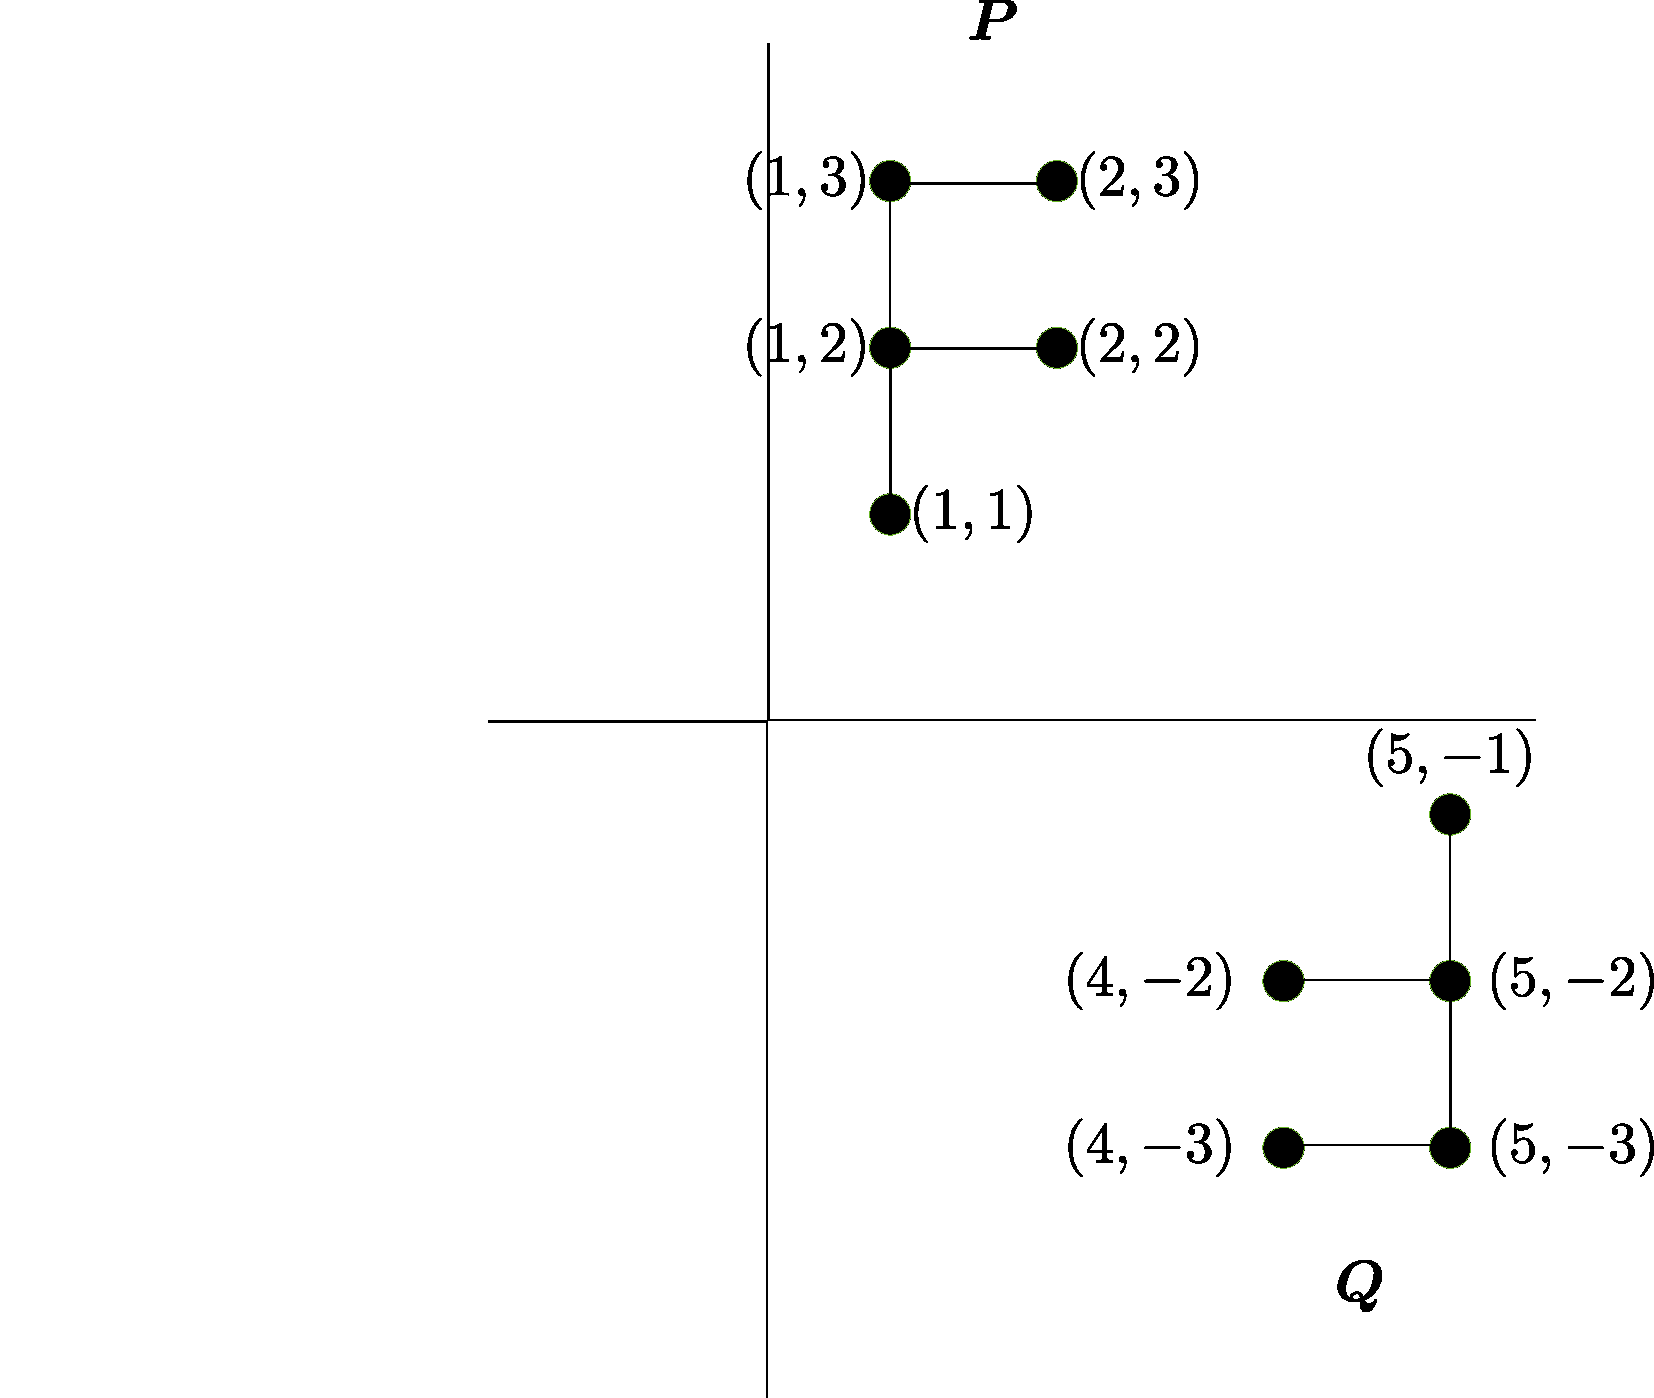
\includegraphics[width=12cm]{fig1.pdf} 
\centering
\caption{denoting set of points of P and Q}
\end{figure}
Let $\vec p_i$ and $\vec q_i$ denote the set of points in $\R^2$ (i.e. $\mat P = \{\vec p_i \} = \{(1,1), (1,2), (2,2), (1,3), (2,3)\}$ and $\mat Q = \{\vec q_i \} = \{(5,-1), (5,-2), (4,-2), (5,-3), (4,-3)\} \in \R^{2}$ ). The optimal transformation that would be required to align the set of points $\mat P$ onto $\mat Q$ would be a rotation of $180\degree$ and a translation of 6 units in the x direction. In matrix notation the information above can be represented as 
\begin{align*}
\mat R &= 
  \begin{bmatrix}
\cos {180} & -\sin{180}\\
\sin {180} & \cos{180}
\end{bmatrix} \\
\vec t &= \begin{bmatrix} 6 \\ 0 \end{bmatrix}
\end{align*}


Now consider two sets of $n$ points $\vec p_i$ and $\vec q_i$ in $\R^d$. You are required to compute the optimal rigid body transformation such that we minimize  $\norm{\cdot}_{L_2}$. The rigid body transformation can be found by minimising the following cost function: 
\begin{align*}
  J(\mat R,\vec t) &= \argmin\sum_{i=1}^{n}\omega_i\norm{(\mat R\vec p_i+\vec t)-\vec q_i}^2
\end{align*}
where $\omega_i$ are the weights and can be arbitrarily chosen.
\begin{enumerate}[label=\alph*.]
    \item Show that the optimal translation is given by $\vec t = \vec{\bar q} - \mat R\vec{\bar p}$ where $\vec{\bar q}, \vec{\bar p} $ represent the weighted centroids of P and Q. 
    (Hint: Assume that $\mat R$ is initially fixed)
    \item Using the value of $\vec t$ from part (a), show that the optimal rigid body transformation is given by 
        \begin{align*}
          J(\mat R) &= \argmin\sum_{i=1}^{n}\omega_i\norm{\mat R\vec\alpha_i - \vec\beta_i}^2
        \end{align*} where $\vec\alpha_i's$ and $\vec\beta_i's$ must be defined by you.
        
    \item Show that the optimal rigid body transformation above can be re-written as 
        \begin{align*}
          \argmax\sum_{i=1}^{n}\omega_i\vec\beta_{i}^{T}\mat R\vec\alpha_i
        \end{align*}
        (Hint: $\mat{R^TR} = \mat I $) 
        
    \item By converting the expression above into matrix notation, show that the summation is equivalent to $tr(\mat{WB^TRA})$ (where $tr(\mat C)$ denotes the trace of $\mat C$ and $\mat W, \mat B, \mat A $ are matrices containing $ w_i's, \vec\beta_i's, \vec\alpha_i's$ respectively). In other words 
    \[\argmax\sum_{i=1}^{n}\omega_i\vec\beta_{i}^{T}\mat R\vec\alpha_i = tr(\mat{WB^TRA}) \]
    
    \item By writing $\mat S = \mat {AWB^T}$, compute its SVD and show that the trace from part d can be written as $tr(\mat{\sum V^TRU})$
    \item Show that in order to maximize the trace above, $\mat R = \mat {VU^T}$
    
    \item What qualifies as a rotation matrix? How would you define a rotation matrix in the context of n dimensions? 
    
    \item Implement and test your algorithm in two- and three-dimensions. State the implicit assumptions in the above formulation for computing the optimal rigid body transformation. You should test your algorithm on wide range of test cases, and state when it may break down

    \item Describe the role of $\omega_i$ and how varying them will, if at all, alter the optimal transformation 
    
    
\end{enumerate}


\item You are given a selection of meshes in the form of a \textit{txt} file. 
\begin{itemize}
    \item You are required to write a parser which reads the txt file and outputs an \textit{obj} file in the current directory. You should assume that the mesh can comprise of both quadrilateral and triangle faces. Use Blender to convert one of the valid obj files to STL file format and send it to the 3d printer in the university.
    \item Write a function which outputs whether the face normals for a given mesh are consistently oriented. If the face normals aren't consistently oriented the function should return a list of faces whose normals are inconsistent. List any assumptions you have made in your algorithm. You should test your algorithm on the meshes provided in \texttt{testMeshes} folder, and state which txt files aren't a valid mesh
    \item Write a function which makes face normals consistent. The function is the previous part will tell you whether there are any inconsistent normals. List any assumptions you make about this algorithm 
    \item  Write a function that outputs the non-manifold edges of a mesh. You should test your algorithm on the meshes provided in \texttt{testMeshes} folder, and state which txt files aren't a valid mesh
    \item Write a function which takes as input lists of vertices and faces of a mesh and outputs a list of faces connected to a vertex. The function should return a dictionary where the key of the dictionary is the vertex id, and the value is the list of faces. Ideally, we want to ensure that the faces attached to a vertex are listed in an anticlockwise manner
    \item Write a function which computes the area of the mesh. You can assume that the mesh only consists of triangles
\end{itemize}

For your convenience we have given you three valid test meshes, namely \texttt{validTriangleMesh.txt}, \texttt{validQuadrilateralMesh.txt}, and \texttt{validTriQuadMesh.txt}. The corresponding obj files can be viewed in Blender. As the names implies, \texttt{validTriangleMesh.txt}, \texttt{validQuadrilateralMesh.txt}, and \texttt{validTriQuadMesh.txt}  comprises of triangles, quadrilaterals, and mix meshes respectively. You are encouraged to create smaller meshes for testing your algorithm.

To make testing easier, we have included a test driver. You should call your functions from the test driver \texttt{test\_meshlib} and test the functionality of each of the above features. You are allowed to define the function signatures as you wish. Usually, you will have multiple \texttt{test\_xxx} functions for a given function.

Please do not change the names of the python files provided to you. Write all your functions in meshlib.py


\end{enumerate}
\end{document}
